\subsection{Additional pre-registered benchmarks}\label{sec:extra}
To test the scope stated above on data not used so far, we ran seven further scenarios whose choice and hypotheses were recorded in the repository before any of them was run (file \texttt{PREREGISTRATION\_R1\_EXTRA.md}): CIFAR-10 with the pretrained ResNet-18 of Section~\ref{sec:real}, where the small-CNN failure was attributed to an uninformative reference model; a text benchmark, AG News with a frozen sentence encoder~\citep{reimers2019sbert} and a two-layer classifier head; and KMNIST and EMNIST (47 classes) with the small CNN. Rotation and label-swap groups are built as before, all hyperparameters are unchanged, and every method was run with five seeds. The only choice made for the new data is the learning rate of the text model, which, as for PACS, was selected with FedAvg on a single-concept federation after standardising the embeddings; this amendment was recorded before any run of the compared methods. Table~\ref{tab:extra} reports all results.

\begin{table}[!htbp]
\centering
\caption{Additional pre-registered benchmarks (40 clients, 5 seeds; columns as in Table~\ref{tab:main}). CIFAR-10 (ResNet): pretrained ResNet-18 as in Section~\ref{sec:real}. PACFL and FedDAG-C need image inputs and are not run on AG News.}\label{tab:extra}
{\scriptsize
\begin{tabular}{l r c c c c c c}
\toprule
Method & n & Acc (\%) & Concept (\%) & Worst-grp (\%) & ARI & K & Conflict (\%) \\
\midrule
\multicolumn{8}{l}{\textit{KMNIST rotation}} \\
DisCo & 5 & 86.9 $\pm$ 0.4 & 75.7 $\pm$ 2.6 & 85.0 $\pm$ 1.3 & 0.96 $\pm$ 0.07 & 4.2 & 0.7 \\
DisCo-noAttach & 5 & 86.8 $\pm$ 0.5 & 75.4 $\pm$ 2.6 & 85.0 $\pm$ 1.3 & 0.94 $\pm$ 0.08 & 4.6 & 0.7 \\
FedAvg & 5 & 74.6 $\pm$ 1.3 & 54.1 $\pm$ 2.0 & 73.0 $\pm$ 1.3 & 0.00 $\pm$ 0.00 & 1.0 & 100.0 \\
Local & 5 & 81.6 $\pm$ 0.8 & 44.4 $\pm$ 1.5 & 79.4 $\pm$ 0.8 & 0.00 $\pm$ 0.00 & 40.0 & 0.0 \\
FedAvg-FT & 5 & 76.4 $\pm$ 0.6 & 53.3 $\pm$ 2.0 & 74.9 $\pm$ 0.7 & 0.00 $\pm$ 0.00 & 40.0 & 0.0 \\
IFCA & 5 & 81.3 $\pm$ 4.2 & 61.1 $\pm$ 12.3 & 78.3 $\pm$ 4.6 & 0.43 $\pm$ 0.44 & 3.8 & 18.5 \\
FeSEM & 5 & 81.4 $\pm$ 3.5 & 61.0 $\pm$ 8.9 & 77.8 $\pm$ 1.9 & 0.34 $\pm$ 0.32 & 4.0 & 20.7 \\
MTCFL & 5 & 83.5 $\pm$ 0.8 & 56.1 $\pm$ 2.2 & 81.7 $\pm$ 1.3 & 0.13 $\pm$ 0.01 & 24.4 & 0.0 \\
FL+HC & 5 & 86.6 $\pm$ 1.1 & 74.3 $\pm$ 5.2 & 85.1 $\pm$ 1.3 & 0.89 $\pm$ 0.22 & 4.0 & 3.0 \\
PACFL & 5 & 81.1 $\pm$ 1.9 & 61.5 $\pm$ 4.0 & 78.7 $\pm$ 1.3 & 0.30 $\pm$ 0.16 & 4.0 & 26.0 \\
StoCFL & 5 & 78.3 $\pm$ 2.2 & 49.8 $\pm$ 0.4 & 75.8 $\pm$ 3.0 & 0.00 $\pm$ 0.04 & 11.4 & 9.8 \\
StoCFL-W & 5 & 80.1 $\pm$ 1.2 & 52.4 $\pm$ 1.1 & 77.4 $\pm$ 1.8 & 0.05 $\pm$ 0.05 & 14.2 & 6.2 \\
FedCCFA & 5 & 76.9 $\pm$ 1.2 & 51.7 $\pm$ 1.9 & 75.3 $\pm$ 1.7 & 0.00 $\pm$ 0.00 & 1.0 & 100.0 \\
FedDAG-C & 5 & 85.6 $\pm$ 1.9 & 72.1 $\pm$ 5.8 & 82.9 $\pm$ 3.6 & 0.76 $\pm$ 0.25 & 4.0 & 8.9 \\
Oracle & 5 & 87.2 $\pm$ 0.3 & 76.7 $\pm$ 1.2 & 85.5 $\pm$ 0.8 & 1.00 $\pm$ 0.00 & 4.0 & 0.0 \\
\addlinespace
\multicolumn{8}{l}{\textit{KMNIST label swap}} \\
DisCo & 5 & 87.3 $\pm$ 0.6 & 76.4 $\pm$ 1.3 & 86.1 $\pm$ 0.9 & 0.95 $\pm$ 0.07 & 4.2 & 0.3 \\
DisCo-noAttach & 5 & 87.3 $\pm$ 0.6 & 76.0 $\pm$ 1.0 & 86.1 $\pm$ 0.9 & 0.93 $\pm$ 0.05 & 4.6 & 0.3 \\
FedAvg & 5 & 75.6 $\pm$ 2.8 & 54.5 $\pm$ 1.2 & 68.9 $\pm$ 4.9 & 0.00 $\pm$ 0.00 & 1.0 & 100.0 \\
Local & 5 & 81.3 $\pm$ 0.9 & 44.3 $\pm$ 1.5 & 79.3 $\pm$ 0.8 & 0.00 $\pm$ 0.00 & 40.0 & 0.0 \\
FedAvg-FT & 5 & 81.6 $\pm$ 1.9 & 62.4 $\pm$ 1.2 & 79.2 $\pm$ 2.3 & 0.00 $\pm$ 0.00 & 40.0 & 0.0 \\
IFCA & 5 & 83.7 $\pm$ 1.1 & 63.2 $\pm$ 5.8 & 81.0 $\pm$ 3.4 & 0.36 $\pm$ 0.18 & 4.0 & 18.4 \\
FeSEM & 5 & 84.3 $\pm$ 2.9 & 62.8 $\pm$ 6.6 & 82.3 $\pm$ 3.8 & 0.36 $\pm$ 0.19 & 4.0 & 22.2 \\
MTCFL & 5 & 83.6 $\pm$ 1.0 & 56.4 $\pm$ 0.9 & 82.1 $\pm$ 1.3 & 0.10 $\pm$ 0.02 & 25.0 & 0.2 \\
FL+HC & 5 & 84.9 $\pm$ 0.8 & 68.0 $\pm$ 4.7 & 82.3 $\pm$ 2.8 & 0.45 $\pm$ 0.22 & 4.0 & 20.7 \\
PACFL & 5 & 76.1 $\pm$ 2.2 & 50.3 $\pm$ 1.6 & 70.0 $\pm$ 2.8 & $-$0.03 $\pm$ 0.03 & 4.0 & 36.7 \\
StoCFL & 5 & 78.6 $\pm$ 2.1 & 51.2 $\pm$ 0.7 & 73.9 $\pm$ 2.8 & 0.00 $\pm$ 0.03 & 10.8 & 9.5 \\
StoCFL-W & 5 & 82.6 $\pm$ 1.4 & 57.6 $\pm$ 1.7 & 80.2 $\pm$ 1.3 & 0.07 $\pm$ 0.06 & 15.8 & 4.7 \\
FedCCFA & 5 & 84.0 $\pm$ 1.2 & 63.2 $\pm$ 1.5 & 82.1 $\pm$ 1.6 & $-$0.00 $\pm$ 0.00 & 1.8 & 95.9 \\
FedDAG-C & 5 & 82.0 $\pm$ 2.0 & 59.8 $\pm$ 2.7 & 77.4 $\pm$ 4.5 & 0.24 $\pm$ 0.06 & 4.0 & 28.6 \\
Oracle & 5 & 87.4 $\pm$ 0.7 & 77.2 $\pm$ 0.8 & 86.0 $\pm$ 0.9 & 1.00 $\pm$ 0.00 & 4.0 & 0.0 \\
\addlinespace
\multicolumn{8}{l}{\textit{EMNIST rotation}} \\
DisCo & 5 & 84.2 $\pm$ 0.6 & 71.2 $\pm$ 1.7 & 82.8 $\pm$ 1.7 & 0.98 $\pm$ 0.04 & 4.4 & 0.0 \\
DisCo-noAttach & 5 & 83.7 $\pm$ 0.6 & 69.9 $\pm$ 1.7 & 82.3 $\pm$ 1.2 & 0.94 $\pm$ 0.04 & 5.6 & 0.0 \\
FedAvg & 5 & 65.1 $\pm$ 0.5 & 41.7 $\pm$ 1.5 & 62.9 $\pm$ 1.3 & 0.00 $\pm$ 0.00 & 1.0 & 100.0 \\
Local & 5 & 74.0 $\pm$ 0.7 & 33.0 $\pm$ 0.5 & 72.0 $\pm$ 2.1 & 0.00 $\pm$ 0.00 & 40.0 & 0.0 \\
FedAvg-FT & 5 & 69.3 $\pm$ 1.9 & 45.2 $\pm$ 1.5 & 65.1 $\pm$ 2.8 & 0.00 $\pm$ 0.00 & 40.0 & 0.0 \\
IFCA & 5 & 78.1 $\pm$ 4.9 & 58.8 $\pm$ 8.9 & 72.1 $\pm$ 8.3 & 0.59 $\pm$ 0.31 & 4.0 & 10.9 \\
FeSEM & 5 & 77.1 $\pm$ 7.5 & 58.7 $\pm$ 14.3 & 72.5 $\pm$ 8.9 & 0.54 $\pm$ 0.45 & 4.0 & 20.3 \\
MTCFL & 5 & 77.4 $\pm$ 0.5 & 46.9 $\pm$ 0.5 & 75.7 $\pm$ 1.6 & 0.13 $\pm$ 0.00 & 23.8 & 0.0 \\
FL+HC & 5 & 84.3 $\pm$ 0.4 & 71.8 $\pm$ 1.1 & 83.0 $\pm$ 0.4 & 1.00 $\pm$ 0.00 & 4.0 & 0.0 \\
PACFL & 5 & 77.4 $\pm$ 1.6 & 57.5 $\pm$ 3.5 & 75.0 $\pm$ 1.2 & 0.48 $\pm$ 0.09 & 4.0 & 16.1 \\
StoCFL & 5 & 74.0 $\pm$ 1.0 & 37.2 $\pm$ 0.9 & 71.5 $\pm$ 2.4 & 0.01 $\pm$ 0.01 & 36.2 & 0.4 \\
StoCFL-W & 5 & 75.4 $\pm$ 1.0 & 39.2 $\pm$ 1.7 & 72.5 $\pm$ 3.2 & 0.02 $\pm$ 0.01 & 37.8 & 0.0 \\
FedCCFA & 5 & 71.0 $\pm$ 1.3 & 44.7 $\pm$ 0.7 & 68.7 $\pm$ 1.2 & 0.00 $\pm$ 0.01 & 8.8 & 64.8 \\
FedDAG-C & 5 & 80.5 $\pm$ 2.7 & 64.5 $\pm$ 5.0 & 76.5 $\pm$ 4.9 & 0.72 $\pm$ 0.20 & 4.0 & 11.0 \\
Oracle & 5 & 84.4 $\pm$ 0.5 & 71.8 $\pm$ 0.9 & 83.2 $\pm$ 0.9 & 1.00 $\pm$ 0.00 & 4.0 & 0.0 \\
\addlinespace
\multicolumn{8}{l}{\textit{EMNIST label swap}} \\
DisCo & 5 & 83.7 $\pm$ 0.9 & 68.7 $\pm$ 2.1 & 82.4 $\pm$ 0.9 & 0.56 $\pm$ 0.22 & 5.6 & 2.4 \\
DisCo-noAttach & 5 & 83.5 $\pm$ 1.0 & 68.0 $\pm$ 2.3 & 82.2 $\pm$ 0.9 & 0.54 $\pm$ 0.21 & 6.4 & 2.2 \\
FedAvg & 5 & 83.0 $\pm$ 1.0 & 71.6 $\pm$ 1.2 & 80.5 $\pm$ 1.0 & 0.00 $\pm$ 0.00 & 1.0 & 100.0 \\
Local & 5 & 73.8 $\pm$ 0.7 & 33.1 $\pm$ 0.7 & 71.8 $\pm$ 2.3 & 0.00 $\pm$ 0.00 & 40.0 & 0.0 \\
FedAvg-FT & 5 & 79.1 $\pm$ 1.3 & 66.6 $\pm$ 1.0 & 76.9 $\pm$ 2.1 & 0.00 $\pm$ 0.00 & 40.0 & 0.0 \\
IFCA & 5 & 82.1 $\pm$ 0.8 & 66.8 $\pm$ 1.4 & 79.5 $\pm$ 1.1 & 0.11 $\pm$ 0.15 & 4.0 & 24.1 \\
FeSEM & 5 & 81.9 $\pm$ 0.7 & 67.5 $\pm$ 1.0 & 79.6 $\pm$ 1.6 & 0.05 $\pm$ 0.04 & 4.0 & 29.7 \\
MTCFL & 5 & 78.4 $\pm$ 0.7 & 48.2 $\pm$ 0.3 & 76.7 $\pm$ 1.9 & 0.06 $\pm$ 0.02 & 25.0 & 0.5 \\
FL+HC & 5 & 83.0 $\pm$ 1.1 & 68.4 $\pm$ 1.3 & 81.2 $\pm$ 1.8 & 0.18 $\pm$ 0.08 & 4.0 & 24.3 \\
PACFL & 5 & 81.4 $\pm$ 1.0 & 66.3 $\pm$ 1.1 & 79.2 $\pm$ 1.5 & $-$0.00 $\pm$ 0.02 & 4.0 & 35.5 \\
StoCFL & 5 & 79.0 $\pm$ 0.6 & 50.8 $\pm$ 1.0 & 77.1 $\pm$ 1.9 & 0.00 $\pm$ 0.02 & 33.8 & 0.8 \\
StoCFL-W & 5 & 79.9 $\pm$ 1.1 & 55.9 $\pm$ 1.2 & 77.4 $\pm$ 3.7 & $-$0.00 $\pm$ 0.01 & 34.4 & 0.6 \\
FedCCFA & 5 & 82.9 $\pm$ 1.0 & 70.0 $\pm$ 1.1 & 81.5 $\pm$ 1.9 & 0.00 $\pm$ 0.01 & 9.0 & 64.0 \\
FedDAG-C & 5 & 81.9 $\pm$ 0.9 & 66.7 $\pm$ 1.1 & 79.7 $\pm$ 0.9 & 0.02 $\pm$ 0.07 & 4.0 & 35.5 \\
Oracle & 5 & 84.8 $\pm$ 0.7 & 72.4 $\pm$ 1.4 & 83.6 $\pm$ 0.7 & 1.00 $\pm$ 0.00 & 4.0 & 0.0 \\
\addlinespace
\multicolumn{8}{l}{\textit{CIFAR-10 (ResNet) rotation}} \\
DisCo & 5 & 81.4 $\pm$ 1.1 & 70.4 $\pm$ 0.7 & 78.4 $\pm$ 1.8 & 0.07 $\pm$ 0.09 & 2.2 & 74.4 \\
DisCo-noAttach & 5 & 81.4 $\pm$ 1.2 & 70.3 $\pm$ 0.8 & 78.4 $\pm$ 1.8 & 0.07 $\pm$ 0.09 & 2.6 & 73.5 \\
FedAvg & 5 & 81.2 $\pm$ 1.0 & 70.3 $\pm$ 0.6 & 78.2 $\pm$ 1.8 & 0.00 $\pm$ 0.00 & 1.0 & 100.0 \\
Local & 5 & 76.2 $\pm$ 1.4 & 45.5 $\pm$ 1.6 & 72.6 $\pm$ 1.6 & 0.00 $\pm$ 0.00 & 40.0 & 0.0 \\
FedAvg-FT & 5 & 77.6 $\pm$ 1.2 & 65.9 $\pm$ 0.3 & 73.0 $\pm$ 2.0 & 0.00 $\pm$ 0.00 & 40.0 & 0.0 \\
IFCA & 5 & 80.0 $\pm$ 1.1 & 66.9 $\pm$ 0.9 & 76.5 $\pm$ 1.4 & $-$0.01 $\pm$ 0.03 & 3.4 & 39.4 \\
FeSEM & 5 & 80.2 $\pm$ 1.0 & 67.7 $\pm$ 0.8 & 77.2 $\pm$ 1.9 & $-$0.01 $\pm$ 0.02 & 4.0 & 31.5 \\
MTCFL & 5 & 79.6 $\pm$ 1.6 & 60.1 $\pm$ 0.9 & 76.2 $\pm$ 1.8 & 0.03 $\pm$ 0.02 & 24.8 & 1.5 \\
FL+HC & 5 & 80.3 $\pm$ 1.0 & 67.4 $\pm$ 0.2 & 77.7 $\pm$ 1.6 & 0.01 $\pm$ 0.06 & 4.0 & 29.9 \\
PACFL & 5 & 81.9 $\pm$ 1.2 & 70.5 $\pm$ 0.5 & 79.0 $\pm$ 1.3 & 0.42 $\pm$ 0.06 & 4.0 & 24.7 \\
StoCFL & 5 & 79.2 $\pm$ 0.6 & 62.9 $\pm$ 3.7 & 76.6 $\pm$ 0.7 & $-$0.00 $\pm$ 0.05 & 7.6 & 28.7 \\
StoCFL-W & 5 & 79.2 $\pm$ 1.4 & 63.1 $\pm$ 1.4 & 76.3 $\pm$ 1.9 & $-$0.02 $\pm$ 0.03 & 12.6 & 9.5 \\
FedCCFA & 5 & 80.3 $\pm$ 1.1 & 68.2 $\pm$ 0.6 & 76.9 $\pm$ 2.6 & 0.00 $\pm$ 0.00 & 1.0 & 100.0 \\
FedDAG-C & 5 & 80.5 $\pm$ 1.3 & 67.0 $\pm$ 0.8 & 77.1 $\pm$ 1.8 & 0.02 $\pm$ 0.03 & 4.0 & 60.6 \\
Oracle & 5 & 83.2 $\pm$ 1.3 & 73.7 $\pm$ 0.6 & 79.9 $\pm$ 1.6 & 1.00 $\pm$ 0.00 & 4.0 & 0.0 \\
\addlinespace
\multicolumn{8}{l}{\textit{CIFAR-10 (ResNet) label swap}} \\
DisCo & 5 & 88.3 $\pm$ 0.8 & 81.9 $\pm$ 0.7 & 87.0 $\pm$ 1.2 & 0.99 $\pm$ 0.04 & 4.0 & 0.2 \\
DisCo-noAttach & 5 & 88.3 $\pm$ 0.8 & 81.9 $\pm$ 0.7 & 87.0 $\pm$ 1.2 & 0.99 $\pm$ 0.04 & 4.0 & 0.2 \\
FedAvg & 5 & 71.6 $\pm$ 3.4 & 56.3 $\pm$ 0.8 & 65.2 $\pm$ 5.5 & 0.00 $\pm$ 0.00 & 1.0 & 100.0 \\
Local & 5 & 82.1 $\pm$ 1.2 & 52.5 $\pm$ 1.7 & 80.3 $\pm$ 1.2 & 0.00 $\pm$ 0.00 & 40.0 & 0.0 \\
FedAvg-FT & 5 & 83.2 $\pm$ 1.4 & 66.8 $\pm$ 2.1 & 79.9 $\pm$ 3.0 & 0.00 $\pm$ 0.00 & 40.0 & 0.0 \\
IFCA & 5 & 82.2 $\pm$ 3.8 & 68.4 $\pm$ 4.6 & 78.1 $\pm$ 4.9 & 0.45 $\pm$ 0.13 & 3.8 & 16.0 \\
FeSEM & 5 & 81.8 $\pm$ 2.5 & 66.5 $\pm$ 4.9 & 76.6 $\pm$ 5.3 & 0.34 $\pm$ 0.17 & 4.0 & 23.0 \\
MTCFL & 5 & 86.2 $\pm$ 0.9 & 71.0 $\pm$ 2.1 & 84.8 $\pm$ 1.2 & 0.11 $\pm$ 0.02 & 26.2 & 0.0 \\
FL+HC & 5 & 86.0 $\pm$ 0.7 & 75.1 $\pm$ 3.7 & 83.6 $\pm$ 1.9 & 0.64 $\pm$ 0.19 & 4.0 & 13.2 \\
PACFL & 5 & 72.3 $\pm$ 2.7 & 54.8 $\pm$ 1.4 & 67.4 $\pm$ 4.4 & $-$0.01 $\pm$ 0.02 & 4.0 & 53.9 \\
StoCFL & 5 & 75.0 $\pm$ 4.3 & 54.7 $\pm$ 3.7 & 70.4 $\pm$ 5.2 & 0.02 $\pm$ 0.03 & 9.0 & 21.8 \\
StoCFL-W & 5 & 84.2 $\pm$ 0.9 & 65.9 $\pm$ 1.2 & 82.6 $\pm$ 1.0 & 0.12 $\pm$ 0.05 & 21.0 & 2.1 \\
FedCCFA & 5 & 85.3 $\pm$ 1.2 & 69.1 $\pm$ 1.5 & 83.2 $\pm$ 1.7 & 0.00 $\pm$ 0.00 & 1.0 & 100.0 \\
FedDAG-C & 5 & 73.8 $\pm$ 4.1 & 57.0 $\pm$ 3.5 & 67.1 $\pm$ 7.1 & 0.03 $\pm$ 0.06 & 4.0 & 67.9 \\
Oracle & 5 & 88.3 $\pm$ 0.8 & 82.0 $\pm$ 0.4 & 87.0 $\pm$ 1.2 & 1.00 $\pm$ 0.00 & 4.0 & 0.0 \\
\addlinespace
\multicolumn{8}{l}{\textit{AG News label swap}} \\
DisCo & 5 & 89.4 $\pm$ 3.2 & 81.5 $\pm$ 5.8 & 84.8 $\pm$ 8.3 & 0.79 $\pm$ 0.21 & 3.4 & 10.5 \\
DisCo-noAttach & 5 & 89.5 $\pm$ 3.1 & 81.5 $\pm$ 5.8 & 85.0 $\pm$ 8.0 & 0.79 $\pm$ 0.21 & 3.6 & 10.2 \\
FedAvg & 5 & 75.2 $\pm$ 6.7 & 55.1 $\pm$ 1.8 & 67.7 $\pm$ 10.5 & 0.00 $\pm$ 0.00 & 1.0 & 100.0 \\
Local & 5 & 89.6 $\pm$ 1.0 & 77.4 $\pm$ 0.8 & 87.9 $\pm$ 2.5 & 0.00 $\pm$ 0.00 & 40.0 & 0.0 \\
FedAvg-FT & 5 & 89.5 $\pm$ 1.0 & 68.1 $\pm$ 2.1 & 87.5 $\pm$ 3.6 & 0.00 $\pm$ 0.00 & 40.0 & 0.0 \\
IFCA & 5 & 87.6 $\pm$ 4.5 & 73.7 $\pm$ 13.3 & 83.4 $\pm$ 6.7 & 0.53 $\pm$ 0.32 & 4.0 & 12.4 \\
FeSEM & 5 & 85.4 $\pm$ 4.7 & 66.9 $\pm$ 7.3 & 81.5 $\pm$ 7.4 & 0.24 $\pm$ 0.14 & 4.0 & 25.5 \\
MTCFL & 5 & 90.5 $\pm$ 0.9 & 81.1 $\pm$ 1.5 & 88.9 $\pm$ 2.6 & 0.11 $\pm$ 0.01 & 24.8 & 0.2 \\
FL+HC & 5 & 87.8 $\pm$ 2.5 & 72.7 $\pm$ 4.1 & 85.2 $\pm$ 3.6 & 0.37 $\pm$ 0.09 & 4.0 & 18.6 \\
StoCFL & 5 & 84.2 $\pm$ 2.7 & 64.6 $\pm$ 6.9 & 79.6 $\pm$ 6.3 & 0.11 $\pm$ 0.15 & 6.2 & 16.9 \\
StoCFL-W & 5 & 89.2 $\pm$ 1.6 & 75.7 $\pm$ 6.6 & 86.9 $\pm$ 3.2 & 0.29 $\pm$ 0.16 & 8.6 & 7.9 \\
FedCCFA & 5 & 90.6 $\pm$ 0.9 & 72.4 $\pm$ 3.1 & 88.7 $\pm$ 3.0 & 0.39 $\pm$ 0.35 & 2.6 & 46.3 \\
Oracle & 5 & 91.6 $\pm$ 0.8 & 87.1 $\pm$ 0.5 & 90.2 $\pm$ 2.0 & 1.00 $\pm$ 0.00 & 4.0 & 0.0 \\
\bottomrule
\end{tabular}
}

\end{table}

\paragraph{Outcomes of the pre-registered hypotheses.} Three of the four predictions of success hold, and the predicted failure occurs. (i) On CIFAR-10 with label swaps and the pretrained network, DisCo-CFL recovers the groups (ARI $0.99$, $\hat\Delta=0.34$) and equals the oracle (88.3\%), against 86.2\% for the best baseline (MTCFL); the best baseline ARI is $0.64$ (FL+HC, given $K$). This confirms the diagnosis of the small-CNN failure on CIFAR-10: with an informative reference model the same label-swap groups are recovered. (ii) On CIFAR-10 rotations the pretrained features do not separate the groups ($\hat\Delta=0.02$) and DisCo-CFL fails (ARI $0.07$), as predicted from rotated CIFAR-100; its accuracy is 0.5 points below the best baseline (PACFL, given $K$). (iii) On KMNIST (rotations and label swaps) and EMNIST rotations, DisCo-CFL recovers the groups (ARI $0.95$--$0.98$) and is within $0.3$ points of the oracle. (iv) Two predictions fail. On EMNIST label swaps ARI is $0.56$: the groups are separated ($\hat\Delta=0.32$), but with 47 classes the per-class signatures are noisy, the smallest pooled linkage within a true group is $0.88<\tau$, and DisCo-CFL over-splits (5.6 clusters, 2.2\% of the conflicting pairs merged). Its accuracy (83.7\%) is still the highest among non-oracle methods, 1.1 points below the oracle. On AG News ARI is $0.79$, just below the pre-registered $0.8$; the separation is small ($\hat\Delta=0.13$, as on Office-Home), and in three of the five seeds two groups are merged into one ($K=3$, ARI $0.62$--$0.70$), while the other two seeds recover the groups (ARI $0.93$ and $1.00$). DisCo-CFL is 2.2 points below the oracle in accuracy; FedCCFA has a higher local accuracy (90.6\% against 89.4\%) but a 9-point lower concept accuracy.

\paragraph{Summary.} Across the seven scenarios the hierarchical comparison gives DisCo-CFL a higher mean accuracy than every baseline, with intervals that exclude zero ($+1.2$ points against FL+HC, the closest, to $+10.7$ against FedAvg; Table~\ref{tab:hier}, part c), and a higher concept accuracy by $4.0$--$27.9$ points. Its failure rate is 23\%, against 54--100\% for the baselines (Table~\ref{tab:failure}). The outcomes follow the separation diagnostic of Section~\ref{sec:theory}: recovery succeeds where $\hat\Delta\ge0.24$ and the within-group linkage stays above $\tau$, and fails where $\hat\Delta$ is near or below $1-\tau$ or where noisy signatures with many classes push the within-group linkage below $\tau$.

\paragraph{Separation predicts success across all benchmarks.} Figure~\ref{fig:separation} puts all 31 scenarios with more than one group together, from every benchmark in this paper. The estimated separation $\hat\Delta$ and the ARI of DisCo-CFL are strongly associated (Spearman $\rho=0.81$, $p<10^{-7}$ over scenario means), and the rule ``$\hat\Delta>1-\tau$'' that Theorem~\ref{thm:rec} suggests classifies the scenarios into successes (ARI $\ge0.5$) and failures correctly in 29 of 31 cases. The two exceptions are borderline: the $15^\circ$ rotation ($\hat\Delta=0.06$, ARI $0.52$) and Office-Home ($\hat\Delta=0.13$, ARI $0.26$). EMNIST label swaps, the one scenario where a clearly separated group is split, are counted as a success at ARI $0.56$. The failures of DisCo-CFL are therefore not erratic: they occur where the condition of the theory does not hold. The diagnostic needs the true groups and is computed after the fact; it explains the results but does not choose the reference model in advance (Section~\ref{sec:discussion}).

\begin{figure}[!htbp]
\centering
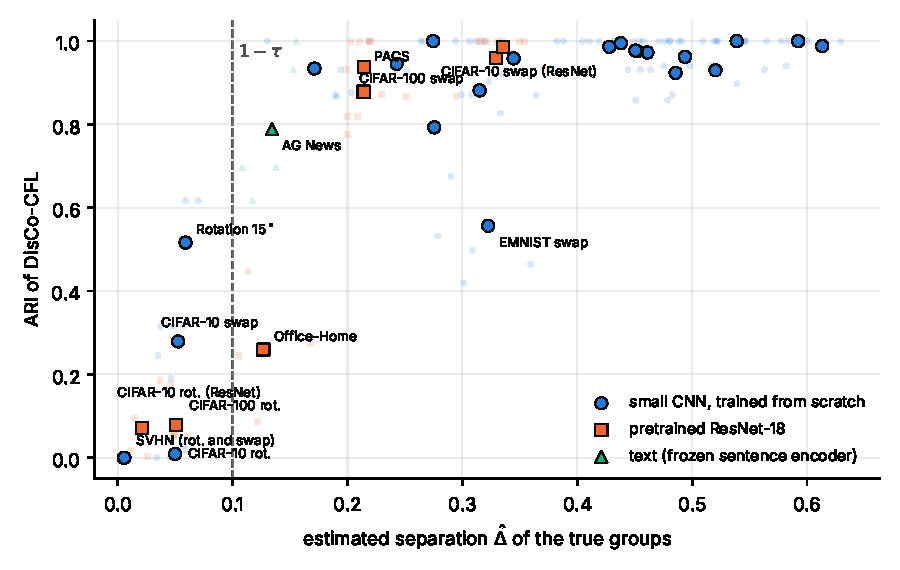
\includegraphics[width=0.85\linewidth]{../results/figures/separation.pdf}
\caption{ARI of DisCo-CFL against the estimated separation $\hat\Delta$ of the true groups, for all 31 scenarios with more than one group (large markers: means over seeds; small markers: individual runs). The dashed line is $1-\tau$, the separation that Theorem~\ref{thm:rec} requires.}\label{fig:separation}
\end{figure}
